\documentclass[mathNotesPreamble]{subfiles}
\begin{document}
\relscale{1.4} %TODO
\section{13.5: Lines and Planes in Space}
  Recall the equation of a line in $\bbr^2$:

  \noindent
  \begin{minipage}{0.5\linewidth}
    \[y=mx+b\]
  \end{minipage}%
  \begin{minipage}{0.5\linewidth}
    \begin{center}
      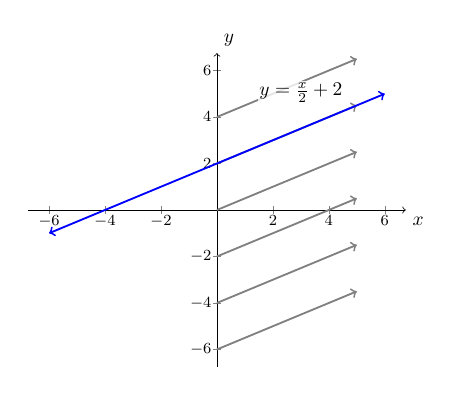
\begin{tikzpicture}[scale=0.7]
        \begin{axis}[
          axis lines=center,
          axis line style={black,->},
          xmin=-6, xmax=6,
          ymin=-6, ymax=6,
          enlargelimits={abs=0.75},
          ticklabel style={font=\footnotesize,inner sep=0.5pt,fill=white,opacity=1.0, text opacity=1},
          xlabel=$x$, xlabel style={at={(ticklabel* cs:1)},anchor=north west},
          ylabel=$y$, ylabel style={at={(ticklabel* cs:1)},anchor=south west},
          every axis plot/.append style={line width=0.95pt, color=blue, samples=100}
          ]
          \foreach \b in {-6,-4,...,4}
            {
            \addplot[->, gray] expression[domain=0:5]{0.5*x+\b};
            }
          \addplot[<->] expression[domain=-6:6] {0.5*x+2} 
            node[black, pos=0.75, above, yshift=12.5pt, fill=white, opacity=0.8, inner sep=0.5pt, text opacity=1] {$y=\frac{x}{2}+2$};
        \end{axis}
      \end{tikzpicture}
    \end{center}
  \end{minipage}%

  where $b$ is the intercept and $m$ is the slope. This idea can be extended into higher dimensions: 
    \[\vecr=\vecr_0+t\vecv\]
  Here, $\vecr_0$ is a fixed point, and $\vecv$ is the position vector that is parallel to the line $\vecr$.
  \begin{center}
    \begin{tikzpicture}[scale=1.0, declare function={
      x0=4; y0=-0.5; z0=4;
      a=-4; b=1; c=-0.5; t=1.4;
      }]
      \begin{axis}[
        axis lines=center,
        axis line style={black,->},
        xmin=-1, xmax=6,
        ymin=-1, ymax=6,
        zmin=-1, zmax=6,
        xmajorticks=false,
        ymajorticks=false,
        zmajorticks=false,
        enlargelimits={abs=0.75},
        view={125}{30},
        every axis plot/.append style={line width=0.5pt, color=blue}
        ]
        \addplot3[<->, domain=-0.75:2.75] (x0+a*\x,y0+b*\x,z0+c*\x);
        \draw[->, shorten >=1.5pt, ClemsonOrange] 
          (0,0,0) -- (x0,y0,z0);
        \addplot3[soldot, black, mark size=1pt] 
          coordinates{(x0,y0,z0)};
        \draw[->, shorten >=1.5pt, ClemsonPurple] 
          (0,0,0) -- (x0+a*t,y0+b*t,z0+c*t);
        \addplot3[soldot, black, mark size=1pt] %TODO Dot missing if out of domain
          coordinates{(x0+a*t,y0+b*t,z0+c*t)};
        \draw[->, shorten >=1.5pt, line width=1pt, BowmanField] 
          (x0,y0,z0) -- (x0+a*t,y0+b*t,z0+c*t);
      \end{axis}
    \end{tikzpicture}
  \end{center}

  \noindent
  \fbox{\parbox{0.9875\linewidth}{
    \textbf{Equation of a Line}\\
    A \textbf{vector equation of the line} passing through the point $P_0(x_0,y_0,z_0)$ in the direction of the vector $\vecv=\bracket{a,b,c}$ is $\vecr=\vecr_0+t\vecv$, or 
      \[\bracket{x,y,z}=\bracket{x_0,y_0,z_0}+t\bracket{a,b,c},\quad \textnormal{for}\quad -\infty<t<\infty\]
    Equivalently, the corresponding \textbf{parametric equations of the line} are
      \[x=x_0+at,\quad y=y_0+bt,\quad z=z_0+ct,\quad\textnormal{for}\quad-\infty<t<\infty\]
  }}

  \noindent
  \fbox{\parbox{0.9875\linewidth}{
    \textbf{Distance Between a Point and a Line}\\
    The distance $d$ between the point $Q$ and the $\vecr =\vecr_0+t\vecv$ is
      \[d=\frac{\abs{\vecv\times \overrightharp{PQ}}}{\abs{\vecv}},\]
    where $P$ is any point on the line and $\vecv$ is a vector parallel to the line.
  }}

  \begin{defn*}[Plane in $\bbr^3$]
    Given a fixed point $P_0$ and a nonzero \textbf{normal vector} $\vecn$, the set of points $P$ in $\bbr^3$ for which \overrightharp{$P_0 P$} is orthogonal to $\vecn$ is called a \textbf{plane} (Figure 13.72)
  \end{defn*}

  \noindent
  \fbox{\parbox{0.9875\linewidth}{
    \textbf{General Equation of a Plane in $\bbr^3$}\\
    The plane passing through the point $P_0(x_0,y_0,z_0)$ with a nonzero normal vector \newline$\vecn=\bracket{a,b,c}$ is described by the equation
      \[a\parens{x-x_0}+b\parens{y-y_0}+c\parens{z-z_0}=0\quad\textnormal{or}\quad ax+by+cz=d,\]
    where $d=ax_0+by_0+cz_0$.
  }}

  \begin{defn*}[Parallel and Orthogonal Planes]
    Two distinct planes are \textbf{parallel} if their respective normal vectors are parallel (that is, the normal vectors are scaling multiples of each other). Two plans are \textbf{orthogonal} if their respective normal vectors are orthogonal (that is, the dot product of the normal vectors is \textit{zero}).
  \end{defn*}

  \pagebreak
  
\end{document}